\chapter{Getting Started}

\section{Game Boy Sound}
The Game Boy sound chip has four channels, each with 4-bit resolution.

\begin{description}
\item[Pulse Channel 1] Square wave with envelope and sweep functions.
\item[Pulse Channel 2] Square wave with envelope function.
\item[Wave Channel] Soft synthesizer, sample playback and speech synthesis.
\item[Noise Channel] Noise with envelope and shape functions.
\end{description}


\section{Key Presses}
In this documentation, key presses are marked up in this fashion:
\begin{description}
\item[\textsc{a}] \textsc{a} button
\item[\textsc{b}] \textsc{b} button
\item[\textsc{start}] start button
\item[\textsc{select}] select button
\item[\textsc{cursor}] any direction of the plus-shaped D-pad
\item[\textsc{left}] D-pad left
\item[\textsc{right}] D-pad right
\item[\textsc{up}] D-pad up
\item[\textsc{down}] D-pad down
\item[\textsc{left/right}] D-pad left or right
\item[\textsc{up/down}] D-pad up or down
\item[\textsc{select+a}] pressing \textsc{a} while holding \textsc{select}
\item[\textsc{select+(b,b)}] pressing \textsc{b} twice, while holding \textsc{select}
\end{description}

\section{Navigating the Program}

\begin{figure}[hbtp]
\centering
\fbox{ 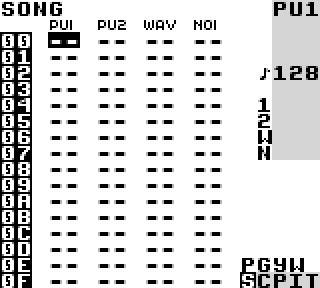
\includegraphics{song} }
\caption{Song Screen}
\label{fig:song}
\end{figure}

Little Sound Dj starts up in the song screen.
The four columns \textsc{PU1, PU2, WAV} and \textsc{NOI} represent the four Game Boy sound channels.
There are two pulse wave channels, one custom wave channel and one noise channel.
Use the D-pad to move the cursor from channel to channel.

\begin{figure}[hbtp]
\centering
\fbox{ 
\includegraphics[width=2.5cm]{map} }
\caption{Screen Map}
\label{fig:map}
\end{figure}

Little Sound Dj has nine screens, arranged in a map shown in the
bottom right of the screen (figure~\ref{fig:map}). 

The most useful screens are placed in the middle row, ordered by level of detail. 
The song, chain and phrase screens are used for sequencing, and work together in a tree-structure
fashion.  The song contains chains, each chain contains phrases, and each phrase contains notes.
They are followed by the instrument and table screens, which are used to create sounds.

To move between the screens, press \textsc{select+cursor}.

\section{Online Help}

\begin{figure}[hbtp]
	\centering
	\fbox{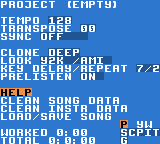
\includegraphics{findhelp}}
	\caption{Project Screen Help}
\end{figure}

To find the in-built help, move to project screen (above song screen) and tap \textsc{a} on \textsc{help}.
The help screen contains key presses for the different screens, as well as a command list.

\section{Making Your First Sounds}
Navigate to the song screen, and move the cursor to the \textsc{pu1} column. Tap the \textsc{a} button,
and a new chain ``00'' will appear.
Edit the chain by pressing \textsc{select+right} to enter the chain screen.
There, tap \textsc{a} to insert a new phrase, then press \textsc{select+right} to go to the phrase screen.

\begin{figure}[hbtp]
\centering
\fbox{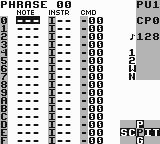
\includegraphics{phrase}}
\caption{Phrase Screen}
\label{fig:phrase1}
\end{figure}

In the phrase screen, you can enter notes to be played back. Move the cursor to the note
column and press \textsc{a} to enter a note. The text C-2 will appear: C being the note, and 2 the
octave. Press \textsc{start} to play the phrase. Notice how the phrase is played back from
top to bottom. You can change the note by holding \textsc{a} and pressing the
D-pad. \textsc{a+left/right} changes the note, and \textsc{a+up/down} changes octave.

Now, try to move the cursor and insert notes on other steps.
To delete a note, press \textsc{a} while holding \textsc{b}.
When you have finished listening, press \textsc{start} again to stop the phrase.

The clean pulse sound might get dull after while. Let's move on to the instrument
screen by pressing \textsc{select+right}.

\begin{figure}[hbtp]
\centering
\fbox{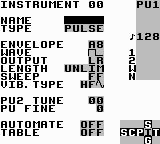
\includegraphics{instr-pulse}}
\caption{Instrument Screen}
\label{fig:instr}
\end{figure}

In the instrument screen, we can make the sound a little bit more interesting.
Try changing the \textsc{env.} and \textsc{wave} fields by moving the cursor there and pressing \textsc{a+left/right}.
As an example, changing the \textsc{env.} setting to \texttt{83} should make the sound shorter.
Press \textsc{start} again to hear the changes as you make them!

The \textsc{type} field sets the instrument type. Instrument types are specific for
channels -- \textsc{pulse} instruments should only be played back in the pulse channels, \textsc{wave} and \textsc{kit}
instruments in the wave channel, and \textsc{noise} instruments in the noise channel.

Let's try out the sampled drum kits. Now, we have to change channel to the wave channel.
Go back to the song screen, move the cursor over to the wave channel, and create a new
chain and a new phrase by tapping \textsc{a}.
Enter a note by tapping \textsc{a}, then \textsc{select+right} to edit the instrument.
Change the instrument type to \textsc{kit} by pressing \textsc{a+right} on the type field,
then go back to the phrase screen. Now, you should be able to enter drum sounds the same way
you entered notes before.

To create new chains and phrases, move the cursor to an empty step in song or chain screen and tap \textsc{a} twice.

\section{Hexadecimal Number System}

Little Sound Dj uses hexadecimal numbers. While the usual decimal number system uses ten digits, 0-9, hexadecimal has 16 unique symbols: the digits 0 to 9, followed by the letters A to F. For clarity, this manual will mark hexadecimal values with a \$ sign.
As an example, let's print a table of numbers -- first with decimal digits, then with
hexadecimal digits\ldots

\begin{figure}[hbtp]
\centering

\begin{tabular}{r|r|r|r|r|r|r|r|r|r|r}
 Decimal & 1 & 2 & 3 & 4 & 5 & 6 & 7 & 8 & 9 & 10 \\
\hline
 Hexadecimal & \$1 & \$2 & \$3 & \$4 & \$5 & \$6 & \$7 & \$8 & \$9 & \$A \\
\end{tabular}

\begin{tabular}{r|r|r|r|r|r|r|r|r|r|r}
 Decimal & 11 & 12 & 13 & 14 & 15 & 16 & 17 & 18 & 19 & 20 \\
\hline
 Hexadecimal & \$B & \$C & \$D & \$E & \$F & \$10 & \$11 & \$12 & \$13 & \$14  \\
\end{tabular}

\end{figure}

Note that the hexadecimal and decimal values are really equal; just the representations differ.
The main reason to use hexadecimal is to save screen space; with hexadecimal
numbers, it is possible to represent every byte value using no more than two digits. (The
byte value range is 0 to 255 -- that is, \$0 to \$FF.)

Representing negative numbers with two digits only can be tricky. In Little Sound Dj,
the numbers are wrapping. That means, when subtracting one from the smallest possible
number (\$0), it will jump to the highest possible value (\$FF). So \$FF can represent -1 as well as 255, depending on the situation.

If this does not make sense -- please don't worry too much -- it will become clear as you spend time with the program.

\section{Initial Troubleshooting}

Does your cartridge not start, crash, or act strange in other ways? Here are some things to try.

\begin{itemize}
	\item To avoid losing songs, always use fresh batteries. Replace as soon as the red light on your Game Boy gets faint, or the screen gets dim.
	\item Clean cartridge pins using a cotton swab and alcohol.
	\item Re-insert the cartridge a couple of times to remove oxide.
	\item Make sure that the cartridge is firmly plugged in. Sometimes it can help to put a piece of tape on the cartridge to give it a snug fit.
	\item Do a full reset of the cartridge memory. This is done by pressing \textsc{select+a+b} on the \textsc{load/save file} button in project screen.
	\item Certain Game Boy Advance/Nintendo DS cartridges do not work with Little Sound Dj. If you have problems with such a cartridge, try one of the Little Sound Dj builds named ``Goomba''.
	\item Search for help on the Little Sound Dj Wiki (\url{http://wiki.littlesounddj.com}) or ask in the Facebook group.
\end{itemize}
